\documentclass[11pt, a4paper]{article}
%\usepackage{proj1}
\usepackage{natbib}
\usepackage{fancyhdr}  
\usepackage{subcaption}
\usepackage{caption}
\usepackage{graphicx}
\usepackage{numprint}
\usepackage{multirow}
\linespread{1.25} 
\setlength{\parindent}{0cm}
\graphicspath{{Images/}}
\usepackage{hyperref}
\usepackage{amsmath}
\usepackage{amsfonts}
\usepackage{amssymb}
\usepackage{amsthm}
\usepackage{mathtools}
\usepackage{commath}
\usepackage{bbm}

%\usepackage[sc,osf]{mathpazo}
\usepackage{subcaption}
\usepackage[a4paper, top=1in, left=1.0in, right=1.0in, bottom=1in, includehead, includefoot]{geometry} %Usually have top as 1in

\usepackage{listings}
\usepackage{color} %red, green, blue, yellow, cyan, magenta, black, white
\definecolor{mygreen}{RGB}{28,172,0} % color values Red, Green, Blue
\definecolor{mylilas}{RGB}{170,55,241}


\hypersetup{colorlinks,linkcolor={black},citecolor={blue},urlcolor={black}}
\usepackage{color}
\urlstyle{same}


\theoremstyle{definition}
\newtheorem{definition}{Definition}[section]

\newcommand{\adja}{q_a}
\newcommand{\adjb}{q_b}
\newcommand{\adjaB}{q_{a,\partial \Omega}}
\newcommand{\adjbB}{q_{b,\partial \Omega}}
\newcommand{\adjB}{q_{\partial \Omega}}
\newcommand{\Adja}{\mathbf{p}}
\newcommand{\Adjb}{q}
\newcommand{\adj}{q}
\newcommand{\Adjc}{{q}_{\partial \Omega}}
\newcommand{\ra}{\rho_a}
\newcommand{\rb}{\rho_b}
\newcommand{\w}{\mathbf{w}}
\newcommand{\f}{\mathbf{f}}
\newcommand{\ve}{\mathbf{v}}
\newcommand{\n}{\mathbf{n}}
\newcommand{\h}{\mathbf{h}}
\newcommand{\K}{\mathbf{K}}
\newcommand{\hr}{\widehat \rho}
\newcommand{\jf}{\mathbf j}

%	\begin{figure}[h]
%		\centering
%		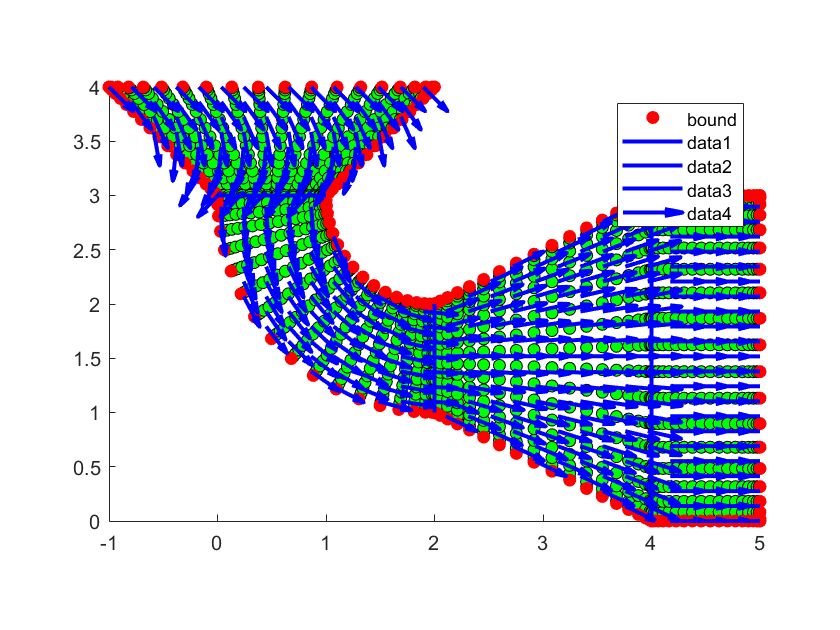
\includegraphics[scale=0.35]{F1.png}
%		\caption{Forward $\rho$ for $a = 0.01$} 
%		\label{F1}
%	\end{figure}

\begin{document}
\section*{ShapeNotes}	
\section{One Dimensional Considerations}
Pseudospectral methods on non-periodic domains are based on polynomial interpolation on non-equispaced points.  
Typically, Chebyshev points $\{x_j\}$ are chosen as collocation points on $[-1,1]$, which are defined as:
\begin{align}\label{defChebyshevPoints}
	x_j= \cos\bigg(\frac{j \pi}{N}\bigg), \quad j=0,1,...,N,
\end{align}	
see \cite{bibTrefethen}.
These points are clustered at the endpoints of the interval, and sparse around $0$. Using this approach, the points are distributed from $1$ to $-1$, which is counter-intuitive. Therefore, in the code library \cite{GoddardPseudospectralCode1}, which is used in producing the results of this report, the Chebyshev points are automatically flipped back to run from $-1$ to $1$. All computations in 2DChebClass are done on this computational domain $[-1,1]$. This can then be mapped onto a physical domain $[a,b]$ of interest vial a linear map.
\\
\\
The function of interest, $f$, is evaluated at the Chebyshev points $\{x_j\}$ and a grid function, $f_j := f(x_j)$, is defined. There exists a unique polynomial of degree $\leq N$ that can be used to interpolate a function $f$ on the grid points $x_j$. The polynomial $p_N$ satisfies, by definition, the following relationship
\begin{align}\label{eqnptov1}
	p_N(x_j)=f_j,
\end{align}
so that the residual $p_N(x_j) -f_j$ is zero at these points. Therefore, this method is called a collocation method, see \cite{Boyd1}. Interpolation on the Chebyshev grid is done using barycentric Lagrange interpolation, derived in \cite{bibTrefethenBerrut1}. The barycentric formula is
\begin{align*}
	p_N(x)= \frac{\displaystyle \sum_{k=0}^N \frac{\tilde w_j}{x-x_j}f(x_j)}{\displaystyle \sum_{j=0}^N \frac{\tilde w_j}{x-x_j}},
\end{align*}
where the weights are defined as
\begin{align*}
	\tilde w_j = (-1)^j d_j, \quad d_j = 
	\left \{
	\begin{tabular}{c}
		$\frac{1}{2}$ \text{for} $j=0$, $j=N$, \\
		$1$ \text{otherwise}, \phantom{abksla} 
	\end{tabular}
	\right .
\end{align*}
see \cite{bibTrefethenBerrut1} and \cite{GoddardPseudospectralCode1}. In the code library 2DChebClass, this is implemented as a matrix-vector product, interpolating from the set of points $\{x_j\}$, onto another set of points $\{x_i\}$, where $i = 0,...., M$ and $j = 0, ...., N$.  The interpolation matrix is of the form
\begin{align*}
	\text{Interp}_{ij} = \frac{1}{\omega_i} \left(\frac{\tilde w_j}{x_i-x_j}\right), \qquad \omega_i = \displaystyle \sum_{k=0}^N \frac{\tilde w_k}{x_i-x_k}.
\end{align*} 
Generally, $\{x_j\}$ lies in computational space $[-1,1]$, while the second set of points lies in computational space by default, but can be customised by the user, to be a set of $M$ points in $[a,b]$. There is another function in 2DChebClass, which takes a set $\{x_j\}$ in physical space instead, but with $N$ points still. This set of points is then first mapped onto the computational domain, using the linear map, before the interpolation matrix is computed, as described above. This method can then be applied to interpolating an arbitrary set of values $\{f_j\}$ onto the new set of points $\{f_i\}$. 
\\
\\
The derivation of the Chebyshev differentiation matrices is described below, following the presentation in \cite{bibTrefethen}. Given a polynomial $p_N$ (++definitely same as above??++), where condition \eqref{eqnptov1} holds, it can be differentiated so that $f'_j = p'(x_j)$, which can be rewritten as a multiplication of $f_j$ by a $(N+1) \times (N+1)$ matrix, denoted by $D$, as follows
\begin{align*}
	f'_j= D f_j,
\end{align*}
using (\ref{eqnptov1}).
A $(N+1) \times (N+1)$ differentiation matrix $D$ has the following entries, compare with \cite{bibTrefethen}
\begin{align*}
	(D)_{00}&= \frac{2N^2 +1}{6},\\
	(D)_{NN}&= -\frac{2N^2 +1}{6},\\
	(D)_{jj}&= -\frac{x_j}{2(1-x_j^2)}, \quad j=1,...,N-1,\\
	(D)_{ij}&= \frac{c_i}{c_j} \frac{(-1)^{i+j}}{(x_i-x_j)}, \quad i \neq j, \quad i,j=0,...,N,
\end{align*} 	
where 
\begin{align*}
	c_i =\left\{\begin{array}{l} 2, \quad i=0 \text{   or   }N, \\1, \quad \text{otherwise.}\end{array}\right.
\end{align*}	
The second derivative is represented by the second differentiation matrix $D_2$, which can be found by squaring the first differentiation matrix; $D_2=D^2$, and more generally the $j^{th}$ differentiation matrix is found as follows
\begin{align*}
	D_j=D^j.
\end{align*}
However, in \cite{GoddardPseudospectralCode1}, the exact coefficients, derived in a similar way as above for $D$, are used to compute $D_2$, since it is more accurate than squaring $D$. Furthermore, all differentiation matrices are derived in computational space and then mapped to physical space using a Jacobian transformation. (++ details?++)
\\
\\
In order to evaluate integrals in a similar way, the so-called Clenshaw--Curtis quadrature is used, which is derived in \cite{ClenCurt1}.
This is, for the integral over a smooth function $f$:
\begin{align}\label{eqnClenCurtQuad}
	\int_{-1}^1 f(x)dx = \sum_{k=0}^N w_kf(x_k),
\end{align}
where the weights are defined as:
\begin{align*}
	w_j = \frac{2d_j}{N}
	\left \{
	\begin{tabular}{c}
		$1- \displaystyle \sum_{k=1}^{(N-2)/2} \frac{2 \cos(2kt_j)}{4k^2-1} - \frac{\cos(\pi j)}{N^2 -1} \quad \quad\text{for $N$ even}$,\\
		$1- \displaystyle \sum_{k=1}^{(N-2)/2} \frac{2 \cos(2kt_j)}{4k^2-1} \quad \quad \quad \quad \quad \quad \ \ \ \text{for $N$ odd}$,
	\end{tabular}
	\right .
\end{align*}
see \cite{GoddardPseudospectralCode1}. In 2DChebClass this is implemented as a vector, such that $(\text{Int})_k = w_k$. Again, this is done in computational space, so that a Jacobian transformation has to be taken to map this onto a desired physical domain. A dot product can be taken between a vector with entries $f_j$ and the resulting integration vector. 
\\
\\
The final aspect to be considered is the convolution matrix, which is needed to compute convolution integrals. 
The convolution integral is defined as:
\begin{align*}
	\left(n \star \chi \right) (y) = \int \chi (y - \tilde y) n (\tilde y) d \tilde y.
\end{align*}
As explained in \cite{GoddardPseudospectralCode1} in detail, $\chi$ is evaluated for all points in the domain at $y - \tilde y$ and transformed into a matrix $\text{diag} \left(\chi\right)$. This is integrated, using the integration vector, to result in the convolution matrix, which can then be applied to a density $n$. This implies that the convolution matrix can be precomputed and applied to different $n$, which saves computational time. 



\section{Two Dimensional Considerations}
In order to extend the definition of the differentiation matrices to two-dimensional grids, a so-called tensor product grid has to be defined. First, Chebyshev points $x_j$, for $j=1,...,n$, on the $x$-axis and another set of Chebyshev points $y_i$, for $i=1,...,m$ on the $y$-axis are taken, both between $[-1,1]$. Then the following two vectors are defined:
\begin{align*}
	\mathbf{x}_{K}=(x_1,x_1,...,x_1,x_2,x_2,...,x_2,...,x_n,x_n,...,x_n)^T,\\
	\mathbf{y}_{K}=(y_1,y_2,...,y_m,y_1,y_2...,y_m,.....,y_1,y_2,...,y_m)^T.
\end{align*} 
In $\mathbf{x}_K$, each $x_j$ is repeated $m$ times, while $\mathbf{y}_K$, each sequence $y_1,y_2,...,y_m$ is repeated $n$ times. The total length of each vector is $n \times m$. 
These vectors are defined, so that the set $(\mathbf{x}_K,\mathbf{y}_K)$ is a full set of all Chebyshev points on the two-dimensional tensor grid.
Note that the points are clustered around the boundary of the two-dimensional grid and sparse in the middle of the grid.
These Kronecker vectors can be used to find the Chebyshev differentiation matrices for two-dimensional problems as follows, compare to \cite{bibTrefethen}. For a first derivative $D$ in the $x$ direction, a Kronecker product is taken of the one-dimensional Chebyshev differentiation matrix with the identity, as demonstrated here with three points:
\begin{align*}
	D_x&=I \otimes D = 
	\begin{pmatrix}
		1 & 0 & 0\\
		0 & 1 & 0 \\
		0 & 0 & 1
	\end{pmatrix}
	\otimes
	\begin{pmatrix}
		d_{11} & d_{12} & d_{13}\\
		d_{21} & d_{22} & d_{23} \\
		d_{31} & d_{32} & d_{33}
	\end{pmatrix}
	\\&=
	\begin{pmatrix}
		d_{11} & d_{12} & d_{13} & & &  & & &\\
		d_{21} & d_{22} & d_{23} & & & & & & \\
		d_{31} & d_{32} & d_{33} & & & & & & \\
		& & &d_{11} & d_{12} & d_{13} & & &\\
		& & &d_{21} & d_{22} & d_{23}  & & &\\
		& & &d_{31} & d_{32} & d_{33} & & &\\
		& & & & & &d_{11} & d_{12} & d_{13}\\
		& & & & & &d_{21} & d_{22} & d_{23}  \\
		& & & & & &d_{31} & d_{32} & d_{33} 
	\end{pmatrix},
\end{align*}
where the block structure matches the repetition of each $x_j$ in $\mathbf{x}_K$.
The second derivative with respect to $x$, $D_{xx}$ can be found by using $D_2$ instead of $D$ in this calculation. 
The derivative with respect to $y$ is found by taking the Kronecker product the other way around:
\begin{align*}
	D_y&=D \otimes I = 
	\begin{pmatrix}
		d_{11} & d_{12} & d_{13}\\
		d_{21} & d_{22} & d_{23} \\
		d_{31} & d_{32} & d_{33}
	\end{pmatrix}
	\otimes
	\begin{pmatrix}
		1 & 0 & 0\\
		0 & 1 & 0 \\
		0 & 0 & 1
	\end{pmatrix}
	\\&=
	\begin{pmatrix}
		d_{11} & & & d_{12} & & & d_{13} & & \\
		& d_{11} & & & d_{12} & & &  d_{13} & \\
		& & d_{11} & & &  d_{12} &  & & d_{13}\\
		d_{21} & & & d_{22} & & & d_{23} & & \\
		& d_{21} & & & d_{22} & & &  d_{23} & \\
		& & d_{21} & & &  d_{22} &  & & d_{23}\\
		d_{31} & & & d_{32} & & & d_{33} & & \\
		& d_{31} & & & d_{32} & & &  d_{33} & \\
		& & d_{31} & & &  d_{32} &  & & d_{33}\\
	\end{pmatrix},
\end{align*}
which now matches the repetition of each $y_1,...y_m$ in $\mathbf{y}_K$.
The Chebyshev differentiation of the Laplacian is given by: $L=I  \otimes D_2 + D_2 \otimes I$.
\\










The advantage of Spectral Methods is that, for smooth functions, the convergence is exponential, see \cite{Boyd1}:
\begin{align*}
	\text{Pseudospectral Error} \approxeq O \bigg[ \bigg( \frac{1}{N} \bigg)^N \bigg].
\end{align*}


A good overview on spectral methods is given in \cite{bibTrefethen} and a more in depth discussion can be found in \cite{Boyd1}.
	
	
	\pagebreak	
	\bibliography{GeneralBib}
	\bibliographystyle{unsrt}
	
\end{document}